% =============================================================================
% =============================================================================
% =============================================================================
\section{The Near-Earth Environment}


From Earth's surface to about \SI{100}{\km}, the atmosphere is a well-behaved fluid: a collisional ensemble of neutral atoms. However, beyond there, its behavior changes dramatically. As altitude increases, solar ultraviolet radiation becomes more intense, which ionizes atmospheric atoms. Density also decreases, slowing collisional recombination. Whereas the neutral atmosphere is held against Earth's surface by gravity, the behavior of charged particles is dominated by Earth's geomagnetic field... and the electromagnetic disturbances created as that field is hammered by the solar wind. 

\todo{Neutral density is larger than charged particle density (?) but it doesn't matter because mean free path is huge. }

The present section outlines the structure of the magnetosphere; that is, the region of space governed primarily by Earth's magnetic field. Particular emphasis is placed on structures which relate closely to field line resonance. 

% -----------------------------------------------------------------------------
% -----------------------------------------------------------------------------
% -----------------------------------------------------------------------------
\subsection{The Outer Magnetosphere}

During quiet times\footnote{Geomagnetically active times are the topic of \cref{sec_storms}}, the behavior of the magnetosphere is driven by the solar wind: a hot, rarefied, fast-moving solar outflow threaded by the Sun's magnetic field\footnote{Usual solar wind velocities, densities, and temperatures fall on the order of \SI{100}{\km/\s}, \SI{10}{\percc}, and \SI{1}{\keV} respectively. At Earth's orbit, the Sun's magnetic field has a magnitude around \SI{1}{\nT}. }. 

The magnetosphere's outer boundary represents a balance between the solar wind dynamic pressure and the magnetic pressure of Earth's dipole field. On the dayside, the dipole is compressed, pushing the magnetopause to within \SI{10}{\RE}\footnote{Distances in the magnetosphere are typically measured in units of Earth radii: $\SI{1}{\RE} \equiv \SI{6378}{\km}$. } of Earth. The nightside magnetosphere is stretched into a long tail which may exceed \SI{50}{\RE} in width and \SI{100}{\RE} in length. 

Consistent with \amplaw, the interplanetary magnetic field is separated from the magnetosphere by a current sheet: the magnetopause. On the dayside, the magnetopause current flows duskward; on the nightside, it flows dawnward around the magnetotail. 

Plasma within the tail is cool (\about\SI{100}{\eV}) and rarefied (\about\SI{e-2}{\percc}). Earth's dipole is significantly deformed in the magnetotail; the magnetic field in the northern lobe of the tail points more or less Earthward, and vice versa. The two lobes are divided by the plasma sheet, which is comparably hot (\about\SI{1}{\keV}) and dense (\about\SI{1}{\percc}). The plasma sheet carries a duskward current which connects to the magnetopause current. 

%In the outer magnetosphere, an important distinction exists between open and closed magnetic field lines. Closed field lines, such as those in the plasma sheet, connect at both ends to the magnetic dynamo at Earth's core. Open field lines, such as those in the tail lobes, meet Earth at only one end; the other connects to the interplanetary magnetic field. 

\todo{Open vs closed field lines. }

\todo{Magnetic flux freezing. }

\todo{Reconnection. Slow accumulation of energy in the tail. }

%In the outer magnetosphere (as well as most of the inner magnetosphere), collisions are so infrequent that magnetic flux is said to be ``frozen in'' to the plasma. Charged particles move freely along magnetic field lines, but cannot cross from one line to another. Compression of the magnetic field is synonymous with compression of the ambient plasma. 

% -----------------------------------------------------------------------------
% -----------------------------------------------------------------------------
% -----------------------------------------------------------------------------
\subsection{The Inner Magnetosphere}

Within about \SI{10}{\RE} of Earth, the dipole magnetic field is not appreciably deformed by the solar wind. 

\todo{Get a better number than \SI{10}{\RE}, either for here or for the position of the magnetopause. }

\todo{Radiation belts. One at L\about2 and another around L\about5. T\about\SIrange{e5}{e6}{\eV}. Density... Radial diffusion... }

\todo{Plasmasphere. Out to L\about4. Density ranges \SIrange{1}{e4}{\percc}. Cold: T\about\SI{1}{\eV}. Plasmapause location is set by balance between... }

\todo{Ring current. L\about2 to 9. T\about\SIrange{e3}{e5}{\eV}. Density... Dst... }

% -----------------------------------------------------------------------------
% -----------------------------------------------------------------------------
% -----------------------------------------------------------------------------
\subsection{The Ionosphere}
  \label{sec_ionos}

\todo{Is this its own section, or should it be folded in with the inner magnetosphere? }

%From \cite{paschmann_2003}: ``In the thermosphere, the solar ultraviolet (UV) light and energetic particles precipitating from the magnetosphere produce ionization increasing with altitude. At the same time the particle density is low enough to make the recombination times of the ionized atoms and molecules sufficiently long to allow a significant fraction of the gas to remain ionized. This produces a conducting layer of the atmosphere known as the ionosphere. The ionosphere begins at $\sim\SI{65}{\km}$, has a peak plasma density between 200 and 300 km, and eventually merges with magnetospheric regions $\sim$1000--2000 km altitudes.''

%One hundred kilometers above Earth's surface, give or take, the neutral atmosphere transitions into the conducting ionosphere. Solar ultraviolet radiation is intense enough -- and collisional recombination slow enough -- to maintain a sizable density of charged particles. Moreover, collisions are common enough to disrupt the plasma's frozen-in condition\footnote{In a collisionless plasma, charged particles move freely along magnetic field lines, but cannot cross magnetic field lines; as a result, a compression in the plasma is synonymous to a compression of the plasma that threads it. }, allowing current to flow perpendicular to Earth's dipole magnetic field. 

%In the ionosphere ($\sim\SIrange{e2}{e4}{\km}$), solar ultraviolet radiation is intense enough -- and collisional recombination slow enough -- to maintain a sizable density of charged particles. 

\todo{``Sweet spot'' where there is a charged population and also a nonzero perpendicular conductivity. Ionospheric currents create magnetic field signatures on the ground. }

\todo{Convection electric field, and two-cell convection. Does $\vec{E}=\cross{V}{B}$ still work when there are collisions? }

\todo{D, E, F layers. Stratification of different species. Ionization by UV radiation, charged particle precipitation, and cosmic rays. }

\todo{Conductivity profiles used in \cref{ch_model}. Tabulated, height-resolved values from Appendix B of Kelley's book\cite{kelley_1989}. Adapted by Lysak\cite{lysak_2013} to account for the latitude-dependent density profile. Also mass loading: mean molecular mass of \SI{28}{\amu} at \SI{100}{\km}, \SI{16}{\amu} around \SI{400}{\km}, down to \SI{1}{\amu} above \SI{1400}{\km}. }

\begin{figure}[H]
    \centering
    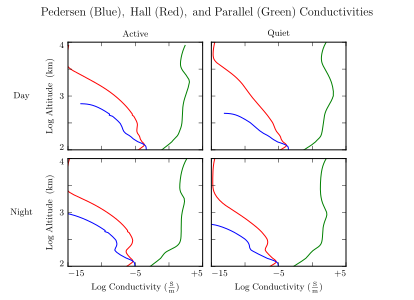
\includegraphics[width=\textwidth]{figures/sigma.pdf}
    \caption[Ionospheric Conductivity Profiles]{
      Ionospheric conductivity profiles, adapted by Lysak\cite{lysak_2013} from Appendix B of Kelley's textbook\cite{kelley_1989}. 
    }
    \label{fig_sigma}
\end{figure}

\todo{Precipitation. Inverted V. Aurorae. }

%The effects of mean molecular mass on conductivity are computed per the usual definitions. 
%\begin{align}
%  \sp &= \displaystyle\sum_s \frac{n_s q_s^2}{m_s} \frac{\nu_s}{\nu_s^2 + \Omega_s^2} &
%  \sh &= -\displaystyle\sum_s \frac{n_s q_s^2}{m_s} \frac{\Omega_s}{\nu_s^2 + \Omega_s^2} &
%  \sz &= \displaystyle\sum_s \frac{n_s q_s^2}{m_s \nu_s}
%\end{align}

\begin{longtable}{ @{\extracolsep{\fill}} lrrr @{\extracolsep{\fill}} }
  \caption[Integrated Ionospheric Conductivity]{Integrated Ionospheric Conductivity (\si{\S})}
  \label{tab_sigma_ionos} \\

  \toprule
  &
  $\Sigma_0$ &
  $\Sigma_P$ &
  $\Sigma_H$ \\
  \midrule
  \endfirsthead

  % Footer for the end of the table
  \bottomrule
  \endlastfoot

  Active Day &
  --- &
  13.0 &
  17.0 \\

  Quiet Day &
  --- &
  5.6 &
  10.2 \\

  Active Night &
  --- &
  0.8 &
  0.3 \\

  Quiet Night &
  --- &
  0.2 &
  0.3 \\

\end{longtable}


